\documentclass[hyperref,english,bachelorofscience,bibnum]{cgvpub}
%weitere Optionen zum Erg�nzen (in eckigen Klammern):
% 
% bibnum	numerische Literaturschl�ssel
% final 	f�r Abgabe	
% lof			Abbildungsverzeichis
% lot			Tabellenverzeichnis
% noproblem	keine Aufgabenstellung
% notoc			kein Inhaltsverzeichnis
% twoside		zweiseitig
\author{Daniel Bekele}
\title{Interactive Registration of 3D Scans in VR}
\birthday{15th January 1995}
\placeofbirth{Jena}
\matno{309845}
\betreuer{Prof. Dr. Stefan Gumhold}
\bibfiles{new_literature_DB}
\problem{
\section{Motivation and Goals:}
When 3D scanning real objects several scans from different views need to be acquired and combined. For high quality reconstruction of a surface model, the relative 3D scanner poses of the different views need to be determined accurately before combining the points from the individual 3D scans. This process is also called registration. The registra-tion problem can be split into coarse and fine registration. In coarse registration a regis-tration with low accuracy is determined which is further refinded by a fine registration, for which fully automatic methods work efficiently. The goal of the thesis is to study the coarse registration problem in an interactive setting where a user adjusts the relative poses in a VR environment and to compare its efficiency with a WIMP based interface, e.g. the one implemented in MeshLab [].
\section{Tasks:}
\begin{itemize}
\item Literature research on registration approach with a focus on interactive and semi-automatic approaches
\item Collection of a representative set of 3D scan collections
\item Design of a VR environment for the interactive registration realizing the concept of a workbench and a natural alignment of the 3D scan collection that needs to be registered in a way the selection of individual scans is efficient.
\item Implementation of VR-based picking and positioning strategy of individual point clouds based on the interaction capabilities of a VIVE VR set.
\item Development and implementation of a strategy to guide the user through the process of registering all scans of a dataset
\item Integration of an automatic fine registration algorithm like SparseICP [].
\item Evaluation of the developed methods in a qualitative user study based on a ground truth dataset provided by the Chair of Computer Graphics and Visualization.
\end{itemize}
\section{Optional Tasks:}
\begin{itemize}
\item Integration of a surface reconstruction algorithm in a background process to preview the reconstructed surface based on the current intermediate registration result
\item Design and implement specific interactions and visualizations that help in a faster or more accurate user based registration
\item Improvement of the realism of the VR environment by integrating detailed and textured 3D models.
\end{itemize}
}
\copyrighterklaerung{Hier soll jeder Autor die von ihm eingeholten
Zustimmungen der Copyright-Besitzer angeben bzw. die in Web Press
Rooms angegebenen generellen Konditionen seiner Text- und
Bild"ubernahmen zitieren.}
\acknowledgments{}
\abstracten{}

\begin{document}
\chapter{Introduction}
In the past 30 Years a rapid development in the field of  virtual and augmented reality took place. The technology itself was not new and invented even earlier, but less affordant for users at home. Due to the lack of computational power of home pcs early systems for VR were not available for most people. With the drop of hardware prices and a rising gaming industry things changed soon and VR reality is now available for early adopters. With the rise of cheaper hardware and the improvments of the last few years it is soon to be expected that VR will gain access to most people.

Virtual reality has the possibility to become a mainstream medium, but its purpose is not restricted to entertainment only. Its capability to produce a replica of normally hard accesseble objects and even interia of humans enables it to provide a perspective view on things that are not seeable otherwise. Even objects that are nonexisting in the real virtual at the given moment can be reprocued and examined with this technology. This property is espiacially usefull for real time CAD applications. In near future there is the chance that designing 3D objects will take place in Virtual Reality rather than on 2D screens that need a projection of the 3D virtual world on a plane.

In order to successfully apply such construction techniques, some basic problems need to be solved first. One of these includes the 3D registration problem, commonly known in the field of computer graphics, as well as robotics, medicine and in CAD Applications.
This thesis goal is to conduct research in previous attempts for solutions of this problems which include user interaction, as well as to develop an interactive 3D registration programm. Finally a user study should provide more usefull insights on the interactive registration process in virtual reality.

\chapter{3D scan registration}
The registration problem is defined as finding the matching transformation for one or more sets of data to match to a target set of data.%BELEG
This task can be splitted into the coarse and fine registration.
In order to work properly, or to achieve faster and better results, most registration algorithms require a coarse registration that is done before the actual algorithm starts. 
\begin{quote}
"Depending on the method used, a quite accurate initial
guess is required because some methods have convergence
problems due to the presence of local minima."\cite{salvi2007}
\end{quote}
Fully automated algorithms for the registration problem mostly need 2 different algorithms for coarse and fine alignment. As an example shown in a paper by Ji \cite{Ji2017} an improved method of the ICP for fine alignment and a genetic algorithm for coarse alignment is used. When examining the research results it is obvious that the focus of current researches lies on fully automated approaches. In difference to my thesis user interaction for registration is kept to a minimum, mostly just used to manually check for registration errors due to local minimas. This is the case in a semi automatic of Chao, who used feature based methods for registration and only to reduce rotation errors the user is involved by chosing the correct rotation.\cite{Chao}

In 1994 the 3D image registration for Validation of several medical scans was proposed along with an interactive coregstration algorithm by an article of Uwe Pietrzy et a\cite{Pietrzyk1994}. The main goal was to align scans of brains with a reference scan in order to detect anomalies, which may indicate a desease of the patient. The corregstration is mainly driven by user interaction and achieved accurate results that put up to the fully automated techniques of that time. At the same time the algorithm was far less restricted than the fully automated techniques, because of user interaction. Figure 2.1 shows the workflow of the application developed by them.
\begin{figure}[htbp]
	\centering
		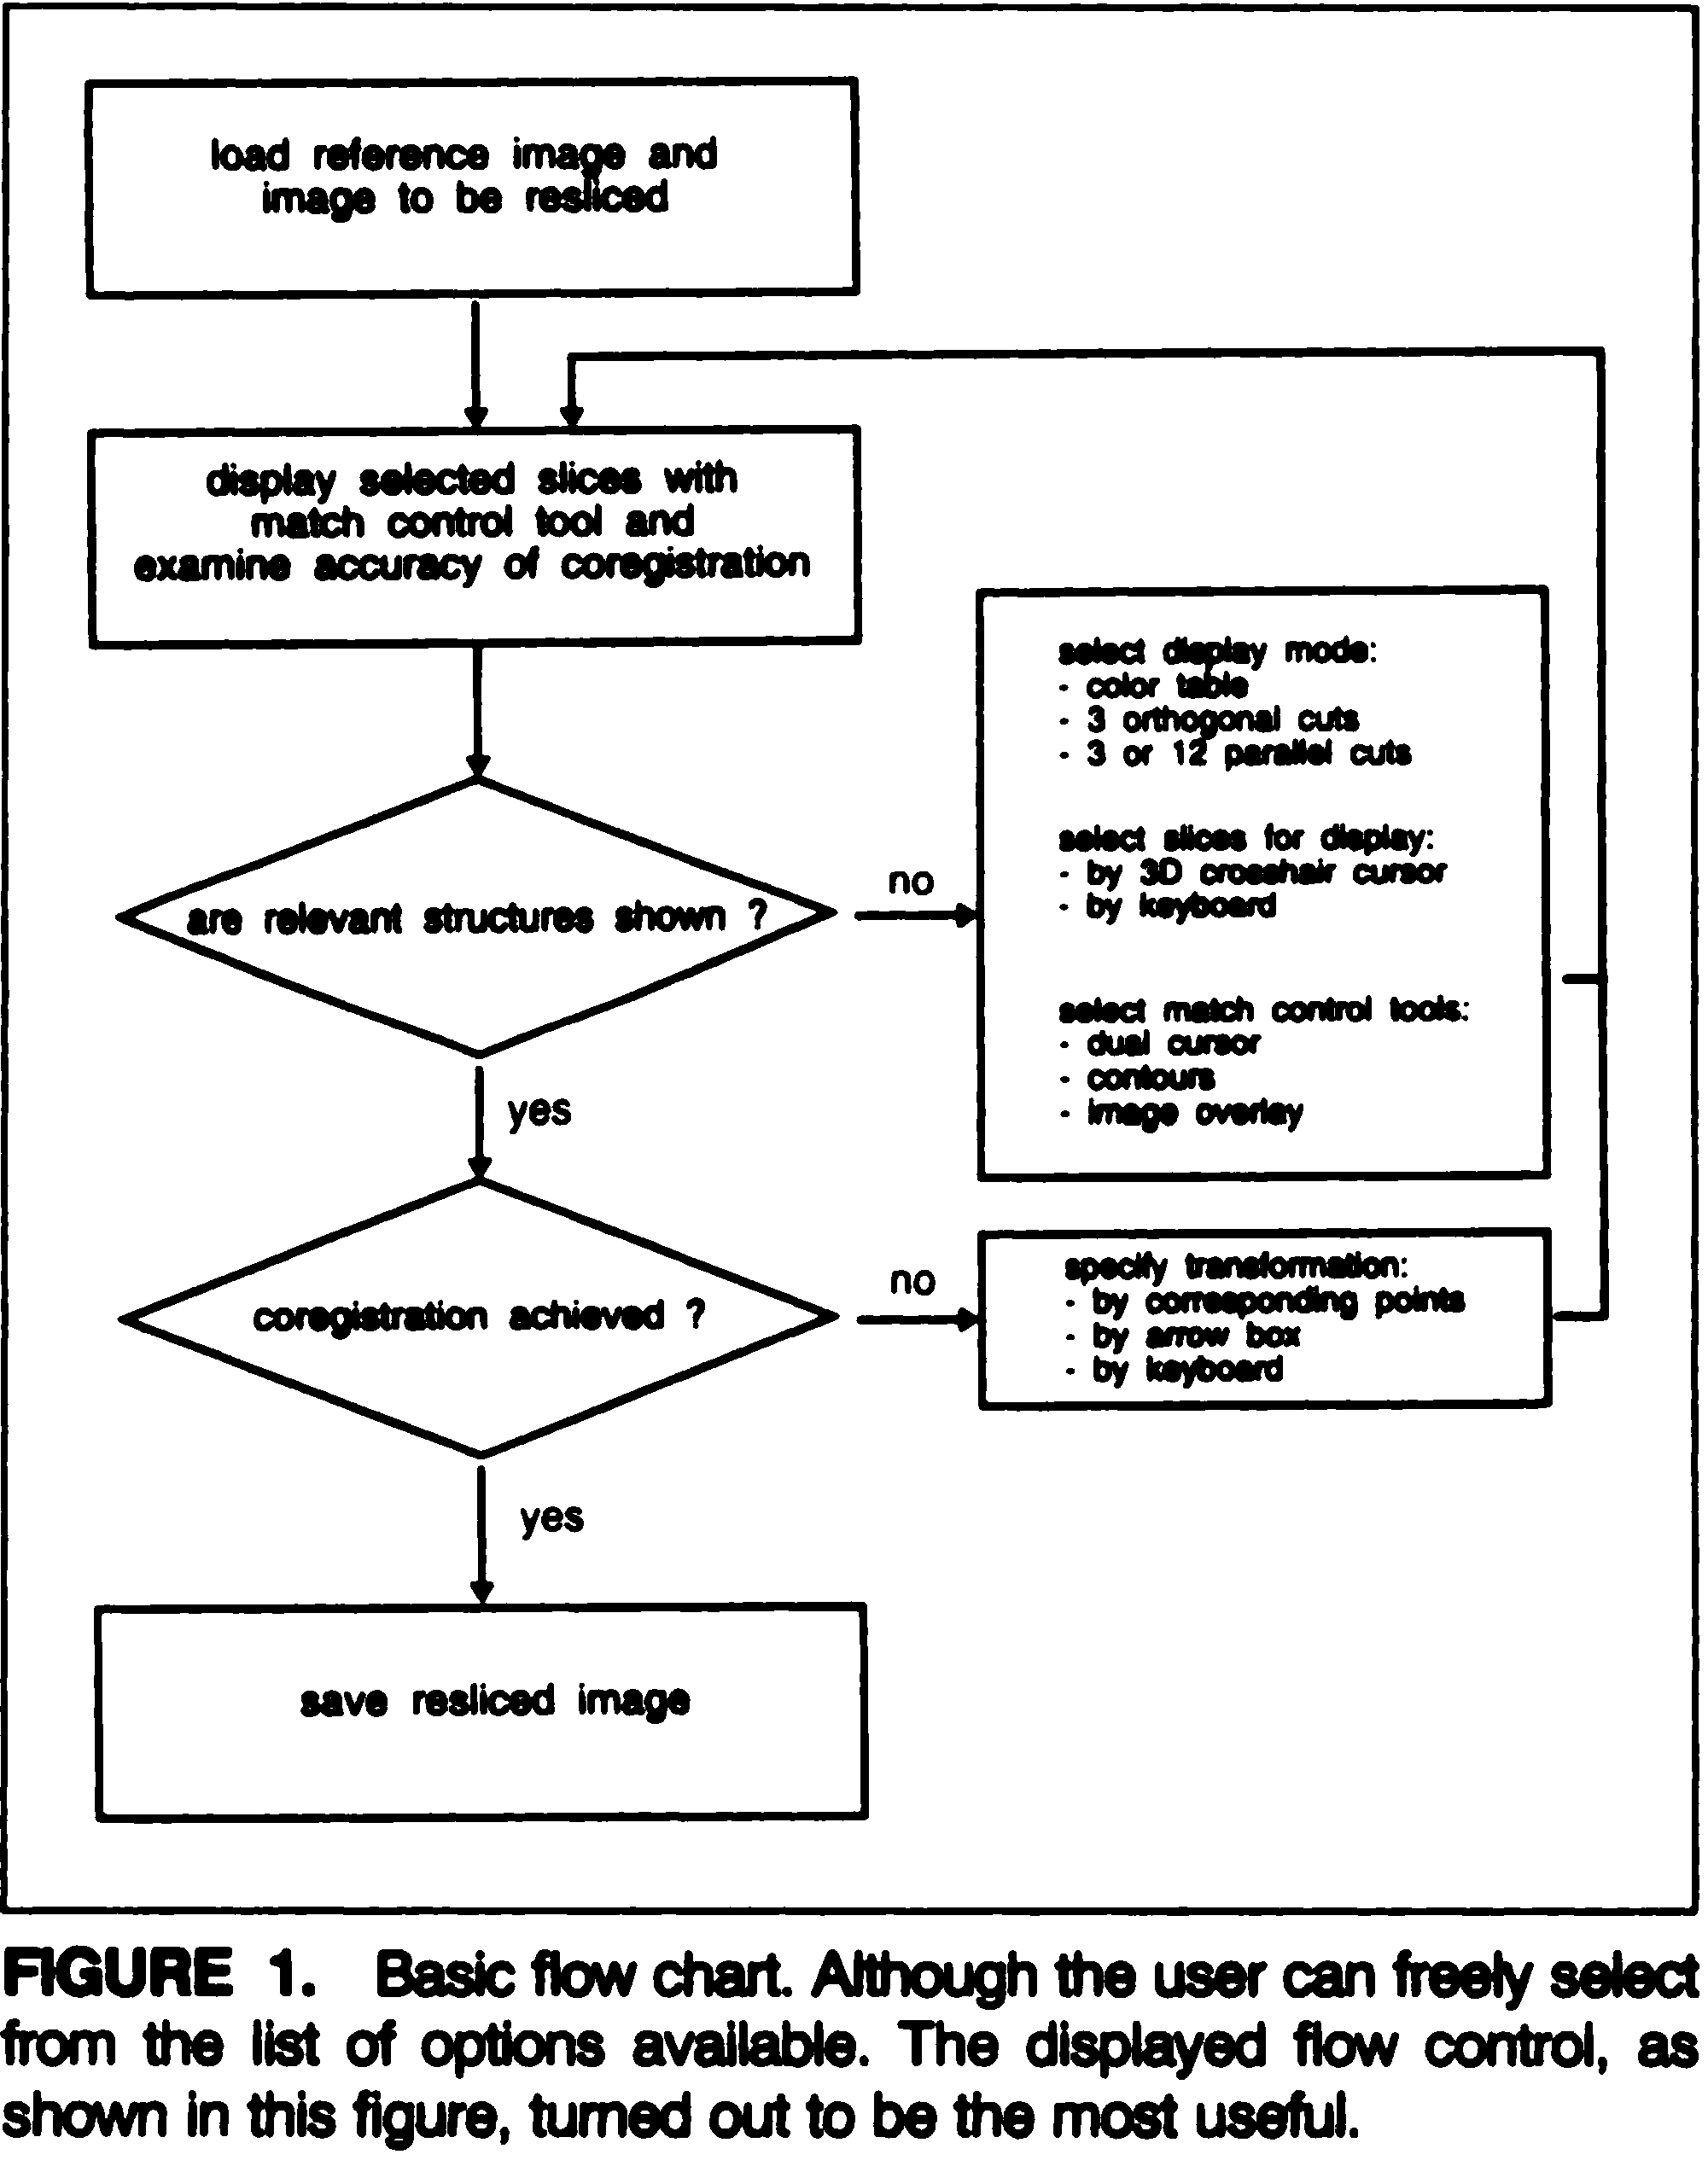
\includegraphics[width= \linewidth]{flow_chart_uwe_p.png}
	\caption{The workflow of the application\cite{Pietrzyk1994}}
	\label{fig:workflow}
\end{figure}

The method proposed by this thesis is a mixture of a manually coarse alignment and simple ICP version that should be capable of running in real time, making it a subject of interest for gaming applictations as well as real time CAD applications.
The coarse registration problem was often solved manually by used a WIMP[explain WIMP] based interface like in Chaos paper \cite{Chao}. To enhance the process further and in order to give the user more insight and controll over his 3D models, a virtual environment is used in our application instead.

The main goal of this thesis is to investigate if this coarse alignment problem can be solved more efficiently by introducing the user to a virtual environment capable of fully displaying the point clouds in all three dimensions, instead of using a WIMP based interface.
The fine registration could then be added with a proper algorithm additionally, in the best case this should execute real time with an animation.

\section{Introduction to registration algorithms}

To achieve this goal of fine registration several steps are necessary:
\begin{enumerate}
\item  Find corresponding points between the roughly aligned sets of data
\item  Find a formula to retrieve the transformation needed to align dataset A to dataset B using the correspondences found in 1.
\item Calculate the actual transformation.
\item Apply the actual transformation
\end{enumerate}

\subsection{Correspondences}

To find corresponding points between 2 sets of points a fast and efficient method is needed, hence the application should work in real time and not use more than 500ms as this is only the first step for the registration algorithm.
The k-nearest neighbour search (knn-search) is commonly used for such problems, as its includes the distances between the nearest points and should deliver good results, given the scans are near together and approximately have the correct rotation. The circumstances of the application fullfill this requirements, since it needs the user to coarse align the scans before the automated fine alignment.
The knn-search does calculate, as its name implies, the distance to the nearest points. To estimate the nearest neighbours, distances between the individual points need to be calculated and then sorted to find the closest points.

Given this situation a simple knn-search with the brute Force method fails. The method would calculate all distances between all points, the resulting complexety of  \textit{O(mnd)} \cite{Garcia2008}, with m as nubmer of all points from point cloud 1 and n with the number of all points from the second point cloud. d is the number of nearest points that are obtained and stored. This does not meet the requirement of the application to work in real time with point clouds with a higher number of points.
To enhance the efficency of this method many different acceleration data structures have been introduced. The one used in the actual implementation of the application for this thesis is the so called KD-tree.

\subsection{KD-Trees}

\begin{quote}
"k-d trees are a generalization of binary search trees."\cite{Nuchter2007}
\end{quote}
In theory this means that all points are represented by a binary tree structure. The root node contains the whole point cloud. The variable k defines the dimensions which is 3 in our example, hence we are working in 3D space when aligning scans. This variable can be higher if e.g. the colours of scans are as additional information availabe.
Building such a tree has an average rutime in the complexity of \mbox{\textit{O(log n)}, to optimize it \textit{O(n log n)}\cite{bentley1975}}.

Their main advantage is their runtime for knn-querys: 
\begin{quote}
"for nearest neighbor queries [empirically observed average running time of \textit{O(log n)}.]" \cite{bentley1975}
\end{quote}
Using KD-trees for a knn-query results in a much better performance since building a kd tree and using it costs less than using brute force method. Furthermore through parallelization the actual runtime can further be reduced. The code excerpt below shows a snippet which uses a KD-tree for a knn-query executing parallel. This implementation is used during the execution of the fine alignment of the version of the ICP this application uses. The code is taken from the stanford university.

\begin{figure}[htbp]
\begin{lstlisting}[frame=trbl]
           /// Find closest point
           #pragma omp parallel for
            for(int i=0; i<X.cols(); ++i) {
               Q.col(i) = Y.col(kdtree.closest(X.col(i).data()));
           }
\end{lstlisting}
\end{figure}

Newer researches have shown that cached KD-trees algorithms using GPU programming have better results\cite{Garcia2008}, this will not be the case in our application since the GPU is fully occupied by providing a rendered stereoscopic view.

The resulting correspondencies can now be used to calculate a rigid-body transformation that aligns two point clouds. To achieve this, the application uses a commonly known algorithm called Iterative closest point (ICP).

\subsection{The iterative closest point algorithm}

\begin{quote}
"ICP starts with two meshes and an initial guess for their relative rigid-body transform, and iteratively refines the transform by repeatedly generating pairs of corresponding points on the meshes and minimizing an error metric."\cite{Rusinkiewicza}
\end{quote}
In this case the Transformation is a translation and a rotation matrix that when applied to the point cloud aligns it to the target point cloud.

The initial guess is provided by the user with a coarse registration. The ICP then makes use of step 2-4 (see top) always iteratively converging to a local optimum.\cite{Besl92}
The ICP algorithm in the variant that was and is widely used in registration problems and was introduced 1992 by P.J. Besl and Neil D. McKay\cite{Besl92}. Over the years several optimization steps have been added to the ICP in order to boost the speed and efficency.

Before starting the actual algorithm it has to be considered that the real time requirement can obviously not be fulfilled with larger point clouds as shown in measurements in table 1 [see table with times]. But aligning and grouping several point clouds to one and aligning this greater point cloud will sooner or later result in a large point cloud that has to be aligned. To still fulfill the real time requirement a subsampling method is needed.

\subsection{Subsampling}

When aligning greater point clouds with more than 1000 Points with an automated registration algorithm, the runtime of these functions in the application do not meet the constraint of running in real time anymore. 
To avoid this problem a subsampling method has been introduced, which uses randomized ranged subsampling. Every point cloud of the group of clouds that is aligned to the target group is counted. The resulting number is divided by the subsampling range. The range indicates that every xth point is sampled. The exact point is randomly chosen in between the ranges distance, counting upwards. The resulting subsampled point cloud is now used for the ICP algorithm, reducing the complexity of the actual task by the factor x.

To avoid large overhead due to the creation of randomized numbers the function uses the default and efficient random Microsoft c++ library <random.h> and only array access with offsets. If the ICP is called again with the same point clouds, the application uses the already stored values, further increasing its efficiency.

Several problems may occur with this method, if no feature extraction, detection of outliers and restriction of subsampling area is defined the accuracy can significantly be lower than without subsampling. Losing features by subsamling causes the algorithm to find less correspondencies, because there are less patterns left. The missing detection of outliers cause them to have greater impact to the resulting alignment, because their amount relative to the totality of points increases. The last point, the restriction of subsampling area is important, because if there are no restrictions, the subsampling method may eject overlapping points of the 2 scans, which are in fact the most important correspondencies for the algorithm. 

\section{Analization and tests of used methods}

In order to enhance the real time compability as well as the general accuracy of the used ICP methods, a public open source code library of the stanford university was used and integrated as header file. Unfortunately this library had a lot of issues with the underlying dependecies and was not perfectly compatible to the framework. As for the sparse ICP implementation results were nowhere near usable, the alignments were diverging instead of getting closer. The basic point to point method which used %which weigting?
was more accurate. Unfortunately this method often failed to align scans due to finding local minima which were incorrect. The missing numerical stability included the possibility to produce INFINITE vectors or even NAN results.

The real time requirement restrained the usage of more complex variants with refined error metrics due to the fact that the running time would increase signiflicantly. Final tests in the actual application with the vive showed that the calculation time increased as well due to the complexity of handling a complete framework which renders a 90Hz stereoscopic view for the vive and has to handle at the same time polled events of the technical devices such as pose events, button events and further more. As the usage of the ICP with more complex scans than the initial test set (the drill scan from the stanford 3D scan repo) completely failed to work in real time with subsampling and even failed to proper align without subsampling, the ICP has been cut out of the program.

\chapter{Interactive VR-Concepts}

\section{The virtual environment}

The virtual environment is defined as the virtual entity that sourrounds the user of a VR technology during the time he is using an HMD. Different to augmented reality which adds an additional layer/interface to the existing reality, letting the user see his natural envirnmont, VR completly sourrounds the user and the actual environment is not visible anymore. What the user can see and percept is solely depended from the created virtual world\cite{Milgram1995}.

This environment should provide orientation in the virtual room as well as interfaces to work in it. The virtual environment is not limited but moving in it is not as easy, as natural movement is restrained to the maximum trackable area of the used VR equipment. 

\subsection{The virtual workspace}

In order to provide the user an appropriate workspace in VR, a virtual room has been designed. The maximum recommended trackable space for the virtual room using the Vive System is a 3.5 meters x3.5 meters quadratic area.
%[https://www.vive.com/us/support/vive/category_howto/what-is-the-recommended-space-for-play-area.html].
To assemble the point clouds efficiently the user has to gather the components and place them on an area. In order to support the users a virtual table has been designed. It is placed in the middle of the room with exact 1m distance to the rooms walls. The resulting size of one meter radius is sufficient for most scans of objects used in this thesis. For a list of used scans and their size see [appendix link]
To avoid cyber sickness or claustrophobic events, the room has only one wall going towards the ceiling. The other 3 sides of the virtual room have smaller fences of about one meter height. They allow sight to the applications background environment. Its task is to emulate more space than there is, to avoid the user feeling trapped in a small 3.5m 3.5m room. The small walls should work as a fence signalling the end of the trackable area. The resulting room can be seen in figure 3.1 in a third perspective view [insert virtual room picture]
 
\subsection{Scaling}

Greater objects may not fit in the room at all and need to be scaled to fit, on the other hand some are so small that the user may have problems to see their important features properly. To give the user the option to adjust his, a scaling function is bound to one of the controllers touchpad and can be used with the drag motion to scale the 3D scan. This has to be done before the actual alignment is done, since scaling is a non homogenus transformation which does not presevere distances between the individual components. The scaling function uses a uniform scale,% transforming the acutal point clouds.

\section{User centred Design for VR}

When building an VR based application, traditional 2D user interface design cannot be simply adapted to 3D.(BELEG!)
Using Popups or mouse emulation projected onto the view frustrum of the user constraints interaction to a 2-Dimensional experience which is rather inefficient, compared to the possibilities VR could provide.
To include VR Technology to the project, especially the cgv-Framework, new user interaction methods have to be provided and tested. Since the user is the active part of the application, controlling the actions and main methods of the scan alignment process, user centred design had to be chosen. 
Human centred design processes for interactive systems, ISO 13407 (1999), states: 
\begin{quote}
"Human-centred design is an approach to interactive system development that focuses specifically on making systems usable."
\end{quote}
%https://www.w3.org/WAI/redesign/ucd
There are many aspects of UCD, the following chapters will focus on the definition and examples used in this thesis corresponding application, showing their usage and further features.

\subsection{Constraints and Affordances}

Affordances describe the relationship between an abstract object or goal a user can achieve with the given actions he has\cite{Jerald2015}.
To improve interaction design it is necessary that these affordances are appropriate and the given actions as easy doable\cite{Jerald2015}.
In our application an affordance would be the relation between moving a scan that has been picked by moving the tracked motion controller. 

Constraints on the other hand are limitations of the given actions a user has. This limitations may be necessary to not confuse the user or to simplify the usage of given methods. A user may move a scan by fault out of the trackable area or below the ground. By adding a simple collision detection that prevents the user from moving scans out of these limitations moving scans is less prone to errors. This would be a constraint to the action of moving the scan with the tracked motion controller. In the application moving scans below zero level is not possible, the scans bounding box is, moved tracked and evaluated. If an action would position any transformed corner point of the box, the translation is stopped and the corresponding controller receives a signal to vibrate. This indicates a violation of physical constraints to the user, preventing him from achieving an unwanted program state with scans hidden below zero ground level. These scans would be invisible.

\subsection{Visual - physical conflict}

By creating constraints to moving objects out of a given space, a user may experience a so called visual-physical conflict. The hand moving the object may go through an area but the application does not apply the physical appropriate result\cite{Jerald2015}.
To avoid or at least lower the impact of this conflict user-feedback can be used to prevent the user from provoking these conflicts by accident, like in the vibrating controller described in the previous chapter.

\subsection{Feedback design}

Feedback is an essential user experience, which should result in information gain about the result or status of a task or object the user interacted with\cite{Jerald}.
A use case in our program would be the switching of colours of a scan when its selected or not. A global selection colour (Bright Red) indicates that this object is selected and will be reference point for further actions. Since scan alignment needs at least 2 scans to be practical the application has a 2 step selection:
Selecting the first scan changes its colour to bright red. But when the next scan is selected the first one changes its colour to a less brighter red signalling it is the secondary pick. Applying the alignment now starts an ICP which moves the second picked scan (the one that is now active) toward the first one.

\subsection{Picking}

Working in VR allows the user to reposition scan components as he wishes to every spot. To align them they need to get close together but if they start already close together they do not look ordered and users tend to split them first, to see the individual scans at least before putting them back together. To solve this problem, all scan components start in a line at a fixed height of about 2 meters at one side of the virtual room. Therefore the user can examine the scans separate.
To pick a scan naturally the user could just walk to the side of the room and pick them up there. This would force one to repeatedly walk across the virtual room to the one wall and back to the table in order to assemble the scan by picking the components. To increase the efficiency and to decrease the effort to reach the scans, the tool has a build in drag function and a corresponding ranged pick function. This function works as a so called "extender grab"\cite{Jerald2015} %[JJ indirekt, Mine at al]
and allows the user via box ray intersection to grab a scan which is out of his personal space.
The hand remote "shoots" a ray from its front direction which now is tested in a Bounding box ray intersection function. If it intersects a component this component is picked.
%Mathematical background?
If there is more than one component in a row that are intersected the one nearest to the user is chosen. 

\subsection{Grouped scans}

During the alignment the user may find the correct rotation and translation to align to scans. To save this but also be able to manipulate the scans rotation and translation without destroying the alignment, the user group scans. These groups now work as one scan with a shared Bounding box and shared translation and rotation and colour. If the user tries to pick the scan they both are selected and if he starts an ICP with the selected group and another group, both scans points are used.
This may come unhandy when the scans are grouped incorrectly and now need to be separated again. To solve this an extra function was implemented. This function splits a group by translating them towards the averaged normal directions of their individual points.
INSERT PICTURE
By using the cross product of their averaged normalized normal vector and a dynamic vector which is generated out of the amount of the amount of components the group has.
This is achieved by dividing a circle by the number of scans. The resulting angle is used in a rotation matrix around the z axis. By multiplying the matrix with the (1,0,0) vector x times normalized directions are derived.
To avoid the possibility that bigger scans can overlap even after the split the minimal distance needed to translate the scans without overlapping is calculated using 2 restrictions:
\begin{enumerate}
\item The maximal Bounding box diagonal is equal to the diameter of a circle around the whole component. To avoid overlapping the point to point distance between the middle points of their bounding boxes has to be at least bigger than the maximal Bounding box Length of the biggest Bounding box
\item The 3 points: averaged middle point of the whole group and the translated Bounding Box middle points of 2 of the scans form a nearly icosceles triangle.
\end{enumerate}
Therefore the minimal translation distance equals (gleichschenkliges dreieck formel).
The application uses a factor of 1.1 of this minimal distance to avoid errors due to the fact that the computer works with floats and doubles which are not always precise and that there may be a distance between the averaged middle point of the group and the middle point of the Bounding Boxes of the scans. This is especially the case if the scans contains outliers.

After this splitting translation was executed, the user now can chose a single component out of the group and separate it. The remaining group turns back to its initial state, the separated scan is lifted above the group.

\subsection{Scan positioning}

When loading a scan into the application there are several problems that occur:
\begin{enumerate}
\item Where should the initial position be when there are no information available?
\item What if the available information are invalid e.g. under the z=0 level?
\item What if the user wants to reset his actions because there are too many errors and he needs to start again?
\item How should positioning be executed without confusing the user with instant teleportation of the components
\end{enumerate}
To solve this problem several functions are introduced to reposition components in different ways.


\subsubsection{The reset function}

This function works as a simple reset. The user forces the components to all disasemble and reposition onto the default wall even if their loading position was somewhere other than default. This function is a hard reset even deleting colour and group information.

\subsubsection{The position above table function}

This function is a repositioning function to reposition a picked group to the middle table in the lowest height available. This height is determined by the lowest corner z-coordinate of the lowest bounding box of the group. Additionally the groups averaged middle point is now in the middle of the table, which is by default the middle of the room.

\subsubsection{The loading functions}

These special functions are not directly called by the user. They are instead called whenever the user decides to change the workspace by loading a new project or directory loading. A newly created component always causes the program to initialize its transformations unless they have a flag set that prevents the program from overwriting the transformations. These flags are used in project files to signalize that this is a component the user has already worked with and this should not be repositioned by loading. 

\subsubsection{The reposition execution animation}

To avoid instant teleportation, every repositioning that is not handled by directly grabbing a component thus attaching it to the hand controller, is instead animated as a linear blend between the original translation position and the target translation position. Additionally a second animation executes the rotation (if there is one) at the same time.
These linear blend is executed on colours as well, making hard colour switches only available for blinking animations or the picking event. This is especially important to signalize that blinking colours are indicating that the user has to confirm an action. Additionally the user can see what he caused with his actions instead of a rapid state change of the program. When several translations are executed by one action it could be irritating with no fluent transition to the new state.(AUSDRUCK)

\subsubsection{The dragging fucntion}

One of the core functionalities for this application is the possibility for the user to directly "grab" a scan and align it by hand next to the target. In order to work this feature needs several helping functions. The picking method determines the selected scan. If the user holds the picking button, the selected scan is now bound to his controller by the controllers virtual pose. This pose is described as a matrix containing the origin point of the controller in world coordinates, as well as all 3 axes of the controllers coordinate system in world coordinates. By calculating the position of the picked group or component in the local coordinate system of the controller and storing this value dragging becomes possible. The local position is obtained by multiplying the local pose of the component (if it is a group all calculations need to be made componentwise seperately) to the inverted pose of the controller. As soon as the pose of the controller changes, the actual pose matrix is multiplied to the already stored local positions, resulting in a tranformation so that the pose of the gourp or scan in the controllers coordinate system remains equal. The actual result in world coordinates is a transformation as if the scan/group is bound to the controllers picking ray. Additionally the user can change the group/scans local pose towards the controllers z axis. This results in the scan/group coming nearer towards the controller, or further away. This action is triggerd by a scrolling movement on the touchpad. 

\subsection{Additional application concepts}

Some features of computer programs have evolved over the time and it is common to include them to all applications because of their general purpose. For example the possibility to restore the program state before the last action is a well known feature and commonly expected to be in every program. (FIND QUOTE)
This feature is implemented by a stack which tracks all program states since the last project loading was called. The inverse function, restoring a state which was after the actual state but has been falsely reversed, is implemented too.(AUSDRUCK!)
The repositioning of scans due to reversing or restoring action triggers an animation as well. This animation is similiar to the one used in the reposition execution animation and applies to colors, rotations and translations.

\chapter{Interactive VR-user study}

\section{Test setup}

\subsection{Equipment}
\subsection{Guidance}

\section{Test results}

\chapter{Evaluation}

\chapter{Problems}

\section{Implementation problems}

The first task was to implement an environment to test and develop the interactive methods used for this study.
However there were several problems that occured during this phase. The real problem was to find a appropriate libary that included a registration algorithm. The application used the version from the stanford university which had strange results when using the sparse ICP version. The results where nowhere near the actual results and about 13 meters away from the right aligment. Possible reasons for this is maybe the use of an older version of the Eigen library in the ICP algorithm. Since this library is incompatible with the framework the only remaining solution was to switch to the ICP algorithm which deliverd better results. Unfortunately this algorithm is nowhere nearly as stable as the sparse ICP algorithm. (BELEG) In order to prevent crashs during execution additional precausons had to be implemented such as check for infinity and NAN vectors, which should normally not occur at this point. The reason is that the ICP is not always numerical stable and can produce such results. Fortunately these are rare and occured only when trying to align point clouds that are not coarse aligned and contained outliers. Since the coarse alignment is taken care of by the user, in the application this problem is minor.

\section{Hardware problems}

When working with VR several individual components have to be taken care of. As for the VIVE HMD from valve, the actual rendering is not done solely by the application, but has to be passed as a render context to the VR compositer, this compositor then renders the pictures for the HMD. The ensurance of compability between both, application and compositor has to be given at any time. Since the development of such applications is not easy this problem caused several delays in the time plan and could not be solved until 2 weeks before the end of this thesis. In detail the driver components for an HMD system have all be written and then linked to the actual application. If the application fails to load any driver the HMD can not connect to the application. To give an example: Even the simple VR example using openGL provided by valve (GITHUBLINK) contains 2000 lines of code, from which are nearly 1200 only initialization functions to start up the actual environment. So all of these functions have to be included and adapted to the own application.



%\section{eine Grafik}
%\begin{figure}[htbp]
%	\centering
%		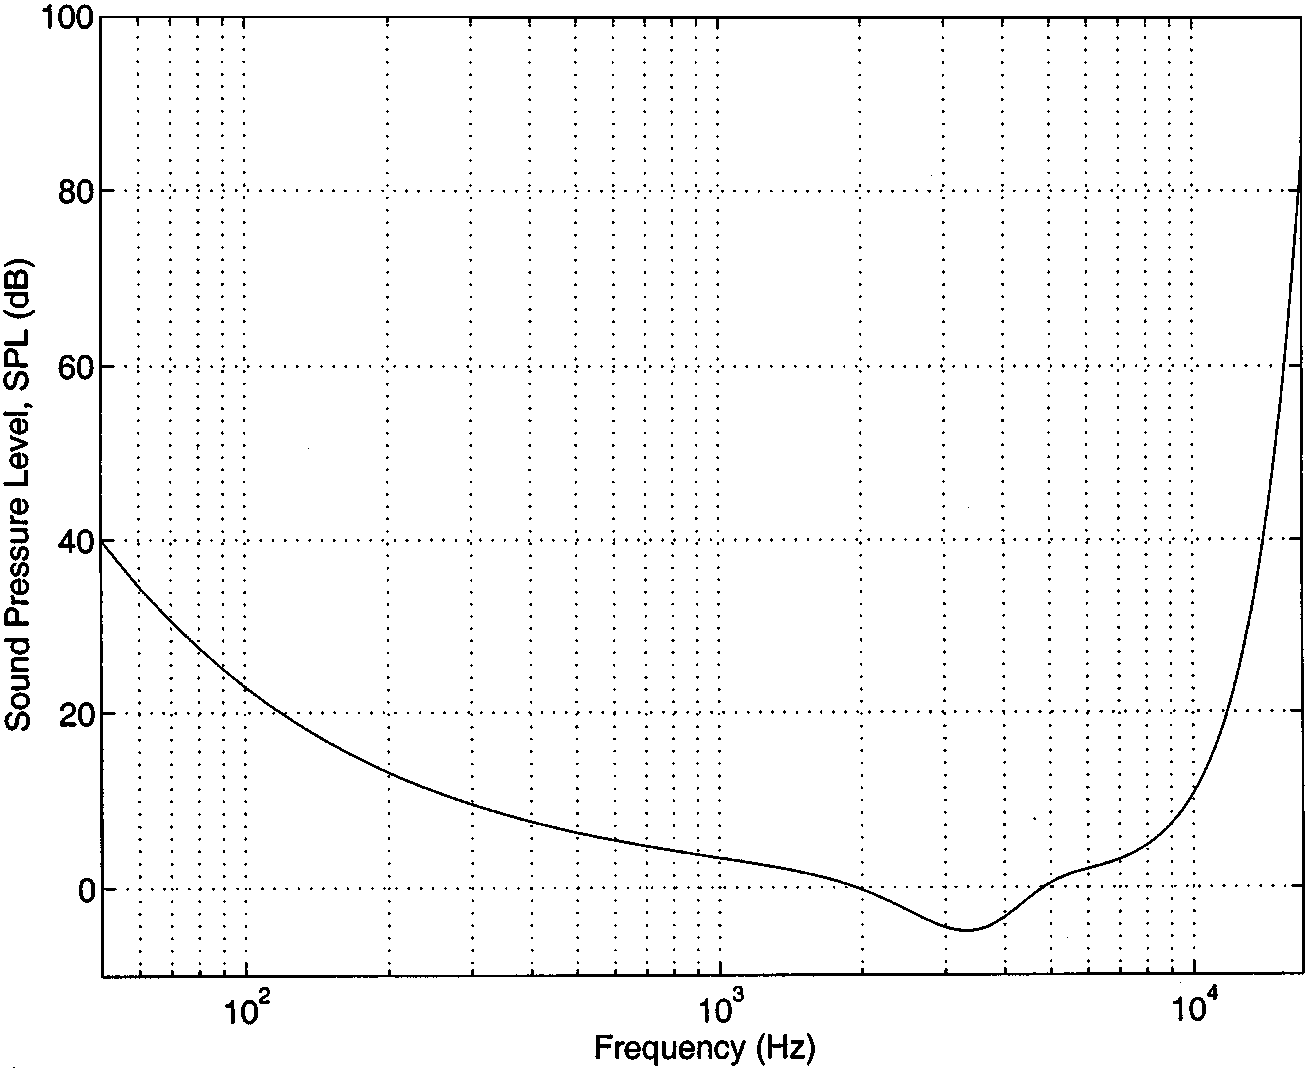
\includegraphics{test.png}
%	\caption{beschriftung}
%	\label{fig:diplominf}
%\end{figure}

\[
\sum_{i=1}^{100}x_i
\]


\cite*{}
\end{document}